%% eval.tex
%% $Id: eval.tex 61 2012-05-03 13:58:03Z bless $

\chapter{Evaluation}
\label{ch:Evaluierung}
%% ==============================

Die Implementierung nichtlinearer Taylormodelle ergibt eine Vielzahl von Konfigurationsmöglichkeiten und damit einen großen Suchraum nach der optimalen Einstellung:
\begin{itemize}
 \item Grenzwert für Cleaning $\delta_c$, Splitting $\delta_s$
 \item Grad der Reduktion durch Sweeping
 \item Anzahl der zu erhaltenden Fehlersymbole
 \item Strategie beim Sweeping
 \item Heuristik für die Reihenfolge, in der Fehlersymbole gesweept werden
 \item Vorgehen beim Splitting
 \item Definition des initialen Taylormodells
\end{itemize}
Diese Konfigurationen werden in \verb+hotm+ als JSON-Datei mit Hilfe einer JSON-Bibliothek\footnote{\url{https://github.com/nlohmann/json} (Stand Dezember 2020)} eingelesen und verarbeitet, um wiederholte Durchläufe mit leicht veränderten Parametern oder Batch-Runs zu vereinfachen. Listing \ref{list:config} zeigt ein Beispiel einer Konfigurationsdatei, mit der versuchsweise 1000 Iterationen der H\e non-Abbildung berechnet werden sollen. 



\section{Housekeeping-Grenzwerte}
Der Grenzwert einer Housekeeping-Methode gibt an ab welchem Wert die jeweiligen Methoden angewandt werden. Bei einem intervall in \verb+hotm+ $[m \pm r]$ mit $m = [c_m \pm \varepsilon_m]$ und $r = [c_r \pm \varepsilon_r]$ als \verb+iRRAM-REAL+s wird
\begin{itemize}
 \item Cleaning angewandt, wenn $\varepsilon_m < \delta_c$ oder $\varepsilon_r < \delta_c$ gilt und
 \item Splitting angewandt, wenn $c_m < \delta_s$ oder $c_m < \delta_s$ gilt.
\end{itemize}
Um diese Werte zu untersuchen, wurde betrachtet, wie sich die Größe des Rechtecks, welches durch die Intervalle $x$ und $y$ aufgespannt wird, abhängig von den Grenzwerten $\delta_c$ und $\delta_s$ auswirkt, beziehungsweise, wieviele Iterationen der H\e non-Abbildung bei einer festen Genauigkeit der \verb+iRRAM-REAL+s möglich sind, bis das Rechteck eine Fläche\footnote{Ab einer Fläche von zirka $2^-{5}$ ist die Überschätzung der Intervalle zu groß und wächst innerhalb weniger Iterationen ($< 10$) gegen $\infty$.} von $>2^{-5}$ erreicht hat.


\begin{table}[tbh]
\centering
\begin{tabular}{ll}
\begin{tabular}{|l|l||c|c|}
\hline \multicolumn{3}{|c|}{\begin{tabular}[c]{@{}c@{}}1000 Bits Präzision \\$x=[0 \pm 2^{-1000}], y=[0 \pm 2^{-1000}]$\\ \end{tabular}}                                                                                                                                                                                                                              \\ \hline
\multicolumn{1}{|c|}{\begin{tabular}[c]{@{}c@{}}$\delta_c$\\($2^{-\delta_c}$)\end{tabular}} & \multicolumn{1}{c||}{\begin{tabular}[c]{@{}c@{}}$\delta_s $\\($2^{-\delta_s}$)\end{tabular}} & \begin{tabular}[c|]{@{}c@{}}Iterationen \end{tabular}   \\ 
\hline
- & - & 451  \\
10   & 10       & 162     \\
10   & 5       & 160      \\
100  & 100      & 273     \\
100  & 50      & 258      \\
500  & 500      & 794     \\
500  & 250      & 746      \\
1000 & 1000     &  1432 \\                                   
1000 & 500    & 1317 \\                                    

\hline 
\end{tabular}
&
\begin{tabular}{|l|l||c|c|}
\hline \multicolumn{3}{|c|}{\begin{tabular}[c]{@{}c@{}}10000 Bits Präzision \\$x=[0 \pm 2^{-10000}], y=[0 \pm 2^{-10000}]$\\ \end{tabular}}                                                                                                                                                                                                                              \\ \hline
\multicolumn{1}{|c|}{\begin{tabular}[c]{@{}c@{}}$\delta_c$\\($2^{-\delta_c}$)\end{tabular}} & \multicolumn{1}{c||}{\begin{tabular}[c]{@{}c@{}}$\delta_s $\\($2^{-\delta_s}$)\end{tabular}} & \begin{tabular}[c|]{@{}c@{}}Iterationen \end{tabular}   \\ 
\hline
- & - & 4360  \\
100  & 100      & 1463     \\
100  & 50      & 1450      \\
1000 & 1000     &  2641 \\                                   
1000 & 500    & 2530 \\           
5000  & 5000      & 7849     \\
5000  & 2500      & 7289      \\
10000 & 10000     &  14455 \\                                   
10000 & 5000    & 13401 \\                                    
\hline 
\end{tabular}

\end{tabular}
\caption[Experimentelle Ergebnisse zu Grenzwerten]{Berechnung der Fläche des Rechtecks mit verschiedenen Grenzwerten für Cleaning $\delta_c$ und Splitting $\delta_s$ und festgelegter Präzision.}
\label{tab:housekeeping}
\end{table}

Tabelle \ref{tab:housekeeping} zeigt experimentelle Ergebnisse für $x_0 = 0 + 1 \cdot \lambda_1 $ und $y_0 = 0 + 1 \cdot \lambda_2$ mit $\lambda_1, \lambda_2 \in [0 \pm \varepsilon]$. Sowohl für 1000, als auch für 10000 Bits Genauigkeit reagiert das Ergebnis sehr sensibel auf die Grenzwerte der Housekeeping-Methoden. Falsch gewählte Werte vergrößern sogar die entstandene Überschätzung, im Vergleich zuer Berechnung ohne Cleaning und Splitting, jeweils in Zeile 1 der Tabellen zu sehen. Werden die Grenzwerte durch die \verb+iRRAM+-Präzision bestimmt, so bleibt der Fehler am längsten klein und die höchste Iterationszahl ist möglich.

\Abbildungps{tbh}{.6}{img/housesteps.png}{fig:housesteps}{Experimentelle Ergebnisse zu Grenzwerten}{Iterationszahl der H\e non-Abbildung mit fester Genauigkeit von 1000 Bits.}

Wie in Abbildung \ref{fig:housesteps} zu sehen ist, hat eine Definition der Grenzwerte unter die zugrunde liegende Genauigkeit keinen Effekt mehr auf die Performanz der Berechnung, da sich die Iterationszahl nicht weiter erhöht.  
 

\section{Sweeping}
 Für eine Sweeping-Konfiguration kommen drei einander beeinflussende Parameter in Betracht: die Sweeping-Strategie, die Gradreduktion und die Anzahl der zu erhaltenen Fehlersymbole. Der Housekeeping-Vorgang für ein Taylormodell inklusive Sweeping besteht wiederum aus vier Schritten:
 \begin{enumerate}
  \item \textbf{(Sweeping)} Reduktion des Taylormodells bis zum angegebenen Grad, je nach Strategie
  \item \textbf{(Sweeping überschüssiger Fehlersymbole)} Entfernen aller Fehlersymbole bis auf die $n$-größten (abhängig von deren Support-Space)
  \item \textbf{(Cleaning)} Verlagern der durch die Schritte 1 und 2 entstandenen Rechenfehler auf der Ebene der \verb+iRRAM-REAL+s auf die Radii der Intervalle
  \item \textbf{(Splitting)} Einführen neuer Fehlersymbole für Monome, deren Koeffizieten durch die Schritte 1-3 zu stark gewachsen sind.
 \end{enumerate}

 Abbildung \ref{fig:sweeping} zeigt die Performanz der Berechnung der H\e non-Abbildung, gemessen an der erreichten Iterationszahl mit statischer Präzision in verschiedenen Fällen. Wie zuvor ist die Berechnung beendet, sobald die Fläche des Rechtecks einen Schwellenwert überschreitet. Zu sehen ist, bei welcher Kombination von Parametern für Sweeing (Schritt 1) und Sweping überschüssiger Fehlersymbole (Schritt 2) die Überschätzung am langsamsten wächst und somit die meisten Iterationen errechntet werden können. Eine Kurve stellt das Ergebnis dar, welches entsteht, wenn $n$ Fehlersymbole erhalten bleiben. Die Zeiteffizienz ist in diesem Falle kein Faktor.
 
Es ist zu erkennen, dass sich die Kurven innerhalb derselben Sweeping-Strategie kaum unterscheiden. Eine Verzehnfachung der Bitzahl in der Breite der Intervalle und der Präzision verzehnfacht auch die erreichte Iterationszahl. 

Die besten Ergebnisse werden beim Beschränken auf \textbf{square\_only} (quadratisches Sweeping) für $n=3$ und Sweeping zum Grade 0; bei \textbf{square\_first} für $n=1$, $n=4$ und Sweeping zum Grade 3 erreicht.

Insgesamt wird jedoch mit \textbf{square\_only} zum Grade 0, also einem Sweeping bis zu einem Taylormodell mit !!!!!!!!, die höchste Iterationszahl erzielt. Im Vergleich mit rein linearen Taylormodellen zeigt sich jedoch eine leichte Verbesserung (siehe Abbildung \ref{fig:extra}). Der Unterschied besteht darin, dass die nichtlinearen Taylormodelle während der Berechnung und besonders während der Multiplikation Punktintervalle erhalten können und sich stattdessen der Grad des Polynoms erhöht. Nach jeder Iteration werden diese dann zunächst zu linearen Taylormodellen reduziert, um dann den Grad durch Splitting auf den Monomen um maximal 1 zu erhöhen. Für lineare Taylormodelle steht lediglich das Splitting für den Kernel zur Verfügung, da sonst nichtlineare Polynome entstünden. Des Weiteren wird hier bereits während der Multiplikation gesweept und Punktintervalle werden zu regulären Intervallen.

Die Performanz des Sweepings \textbf{square\_only} zum Grade 0 verbessert sich im Schnitt mit einer wachsenden Zahl der zu erhaltenen Fehlersymbole, wie in Abbildung \ref{fig:extra} zu sehen ist. Jedes Fehlersymbol erhöht die Menge an erhaltener Abhängigkeitsinformation und sorgt dafür, dass ein Taylormodell dessen runde Ränder besser beschreiben kann. Allerdings stellt die Pratkikabilität dieser Herangehensweise ein Problem dar, da so sehr große Polynome entstehen, die während einer Iteration der H\e non-Abbildung exponentiell in ihrer Länge wachsen.
 
\begin{figure}[tbh]
\centering
\begin{subfigure}{.5\textwidth}
  \centering
  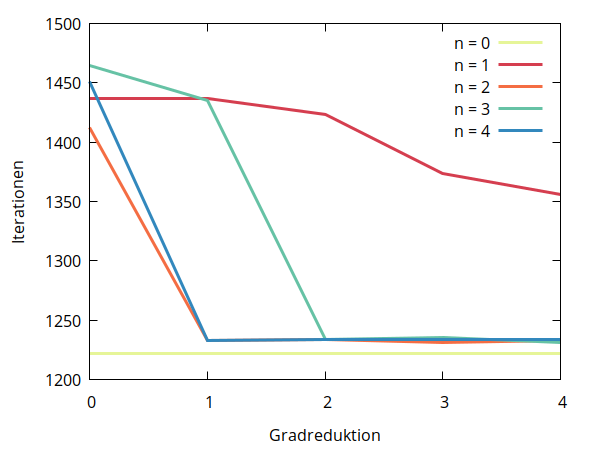
\includegraphics[width=\linewidth]{img/sweeping_only.png}
  \caption{Sweeping beschränkt \textbf{square\_only}}
  \label{fig:sub1}
\end{subfigure}%
\begin{subfigure}{.5\textwidth}
  \centering
  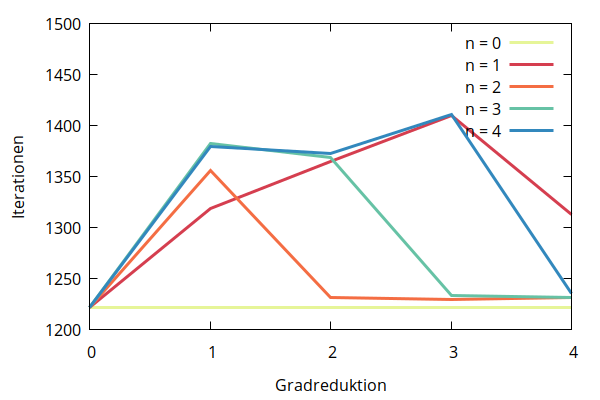
\includegraphics[width=\linewidth]{img/sweeping_first.png}
 \caption{Sweeping beschränkt \textbf{square\_first}}
  \label{fig:sub2}
\end{subfigure}

\begin{subfigure}{.5\textwidth}
  \centering
  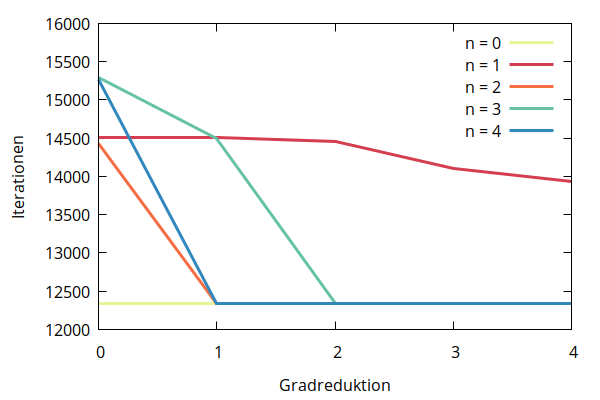
\includegraphics[width=\linewidth]{img/sweeping_only10k.png}
  \caption{Sweeping beschränkt \textbf{square\_only}}  
  \label{fig:sub1}
\end{subfigure}%
\begin{subfigure}{.5\textwidth}
  \centering
  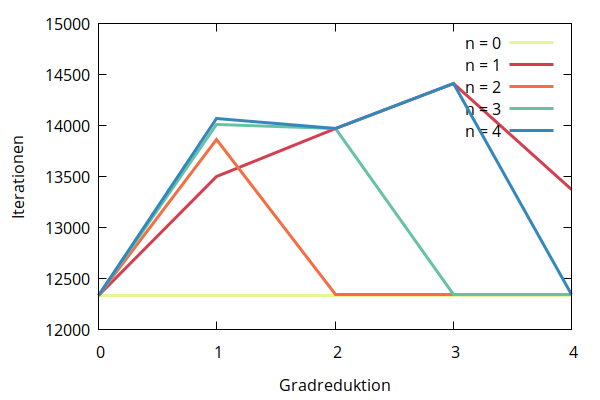
\includegraphics[width=\linewidth]{img/sweeping_first10k.png}
 \caption{Sweeping beschränkt \textbf{square\_first}}
  \label{fig:sub2}
\end{subfigure}


\caption[Sweeping mit verschiedenen Graden]{Anzahl an Iterationen, bis das Rechteck eine gewisse Fläche überschreitet, bei einer festen Präzision und Entfernen aller Fehlersymbole bis auf die n größten. Bei n = 0 bleibt Fehlersymbol erhalten. \\ (a) und (b): Präzision $2^{-1000}$ und ein initiales Rechteck von $x_0 = y_0 = [0 \pm 2^{1000}]$ \\ 
 (c) und (d): Präzision $2^{-10000}$ und ein initiales Rechteck von $x_0 = y_0 = [0 \pm 2^{10000}]$
}
\label{fig:sweeping}
\end{figure}

 \Abbildungps{tbh}{.6}{img/extra.png}{fig:extra}{Experimentelle Ergebnisse zu erhaltenen Fehlersymbolen}{Iterationszahl der H\e non-Abbildung mit fester Genauigkeit von 1000 Bits.}

 
 

%%% Local Variables: 
%%% mode: latex
%%% TeX-master: "thesis"
%%% End: 
